% \documentclass[a4paper,11pt,oneside,notitlepage,pagesize,headsepline,footnosepline,parskip]{scrartcl}

%Schriftgröße, Layout, Papierformat, Art des Dokumentes
\documentclass[11pt,oneside,a4paper,parskip]{scrartcl}

%Einstellungen der Seitenränder
\usepackage[left=3cm,right=2cm,top=1cm,bottom=2cm,includeheadfoot]{geometry}

%neue Rechtschreibung
\usepackage[german]{babel}

%Umlaute ermöglichen
\usepackage[utf8x]{inputenc}

\usepackage{amsmath}
\usepackage{amsfonts}
\usepackage{amssymb}
\usepackage{amsthm}
\usepackage{caption}
\usepackage{multicol}
\usepackage{subfigure}
\usepackage{xcolor}
\usepackage{fontenc}
\usepackage{graphicx}
\usepackage{epstopdf}

\usepackage{setspace}
\usepackage{fancyvrb}
\usepackage{tabularx}

\usepackage{float}

% \usepackage{times}
% \usepackage[T1]{fontenc}

\usepackage{enumitem}

\author{Sebastian Nuck, Benjamin Block}
\title{Semesterprojekt Cluster-Computing}
\subtitle{Dokumentation}
\date{\today}

%Kopf- und Fußzeile
\usepackage{fancyhdr}
\pagestyle{fancy}
\fancyhf{}

%Kopfzeile links bzw. innen
\fancyhead[L]{\nouppercase{\leftmark}}
%Kopfzeile rechts bzw. außen
\fancyhead[R]{Sebastian Nuck, Benjamin Block}
%Linie oben
\renewcommand{\headrulewidth}{0.5pt}

%Fußzeile mittig
\fancyfoot[C]{\thepage}
%Linie unten
\renewcommand{\footrulewidth}{0pt}

\usepackage{listings}
\lstset{
        basicstyle=\small\ttfamily, % Standardschrift
        numbers=left,               % Ort der Zeilennummern
        numberstyle=\tiny,          % Stil der Zeilennummern
        stepnumber=1,               % Abstand zwischen den Zeilennummern
        numbersep=5pt,              % Abstand der Nummern zum Text
        tabsize=4,                  % Groesse von Tabs
        extendedchars=true,         %
        breaklines=true,            % Zeilen werden Umgebrochen
        keywordstyle=[1]\textbf,    % Stil der Keywords
        keywordstyle=[2]\textbf,    %
        keywordstyle=[3]\textbf,    %
        keywordstyle=[4]\textbf,    %
        stringstyle=\color{stringcolor}, % Farbe der String
        showspaces=false,           % Leerzeichen anzeigen ?
        showtabs=false,             % Tabs anzeigen ?
        showstringspaces=false,      % Leerzeichen in Strings anzeigen ?
        framexleftmargin=5mm, frame=shadowbox, rulesepcolor=\color{black}
}
\lstloadlanguages{% Check Dokumentation for further languages ...
	bash,
	[ANSI]C
}

\begin{document}
\setlist{itemsep=0pt,topsep=2pt,parsep=2pt}

\maketitle
\tableofcontents

\section{Projektaufgabe}

Die bearbeitete Aufgabe entspricht der zweiten der zur Verfügung stehenden Aufgaben: \textit{Zusammenhängende Komponenten}.

Zum Programmstart ist eine Matrix mit schwarzen und weißen Feldern gegeben (jedes Feld der Matrix kann als Pixel auf einem Bild aufgefasst werden). Ziel des Programms ist es, alle maximalen zusammenhängenden schwarzen Komponenten (eine Gruppe von schwarzen Feldern) zu finden. Eine Komponente gilt dann als zusammenhängend und maximal, wenn es in den umgebenden Feldern (direkt angrenzend) keine weiteren schwarzen Felder mehr gibt. Eine genaue Definition ist in der ausgegebenen Aufgabenstellung zu finden.

Ausgeben soll das Programm alle gefundenen maximalen schwarzen Komponenten, ihre Größe und eine exemplarische Koordinate in der Matrix (um sie beispielsweise lokalisieren zu können).

Ein Beispiel ist in Abb. \ref{fig:inputbsp} auf Seite \pageref{fig:inputbsp} zu sehen. In der angegebenen Matrix sind 4 maximale schwarze Komponenten mit den Größen 5, 5, 7 und 8. Exemplarische Koordinaten für die Komponenten sind $\{(0, 1), (5, 1), (1, 7), (1, 11)\}$ (beschrieben als Matrix-Indizes, nicht als kartesische Koordinaten).

\begin{figure}[tbhp]
	\centering
	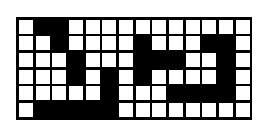
\includegraphics[width=0.7\textwidth]{images/inputbsp.eps}
	\caption{Beispielmatrix wie sie das Programm erwartet}
	\label{fig:inputbsp}
\end{figure}


\section{Aufbau des Programms}

Das Programm ist in 3 wesentliche Schritte eingeteilt:

\begin{enumerate}
	\item Einlesen / Verteilen der Matrix
	\item Ermitteln der maximalen zusammenhängenden Komponenten im lokalen Bereich der Matrix
	\item Übermitteln der Ergebnisse an einen Nachbarn
\end{enumerate}

\subsection{Einlesen, Verteilen}

Nach dem Programmstart wird die Matrix vom Dateisystem des Root-Prozesses eingelesen. Dafür wird die Datei als Parameter beim Programmaufruf angegeben. Anschließend teilt der Root-Prozess die Matrix in möglichst gleich große Teile und verschickt diese an die anderen Prozesse im Cluster. In der aktuellen Programmversion teilt der Root-Prozess die Matrix immer in Streifen. Falls dabei die Anzahl der Matrix-Spalten nicht durch die Anzahl der Prozessoren teilbar ist, wird der Rest dem letzten Prozess zugeteilt (siehe Abb. \ref{fig:matrix_zerteilung} auf Seite \pageref{fig:matrix_zerteilung}).

\begin{figure}[tbhp]
	\centering
	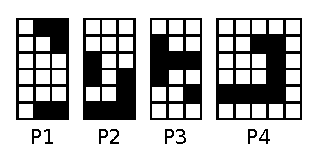
\includegraphics[width=0.7\textwidth]{images/matrix_split.eps}
	\caption{Beispiel für die Zerlegung einer Matrix zur Laufzeit}
	\label{fig:matrix_zerteilung}
\end{figure}

Durch diese Aufteilung kann ein Ungleichgewicht zwischen dem letzen und den restlichen Prozessen entstehen. Da der letzte Prozess aber auch derjenige ist, der am längsten auf seine Vorgänger warten muss, ensteht keine wesentliche Verzögerung im Programmablauf.

Eine zukünftige Version sollte außerdem auf die Eingabedimensionen der Matrix Rücksicht nehmen. Für den Fall, dass die Zeilenanzahl größer als die Spaltenanzahl ist ($m > n$), sollte das Programm die Matrix horizontal zerlegen, damit die Ränder möglichst klein bleiben.

\subsection{Ermitteln der lokalen Komponenten}

Im nächsten Schritt führt jeder Prozessor im Cluster den Kern-Algorithmus mit der empfangenen Matrix aus (siehe Abschnitt \ref{algorithm:find_components} auf Seite \pageref{algorithm:find_components}). Als Rückgabe erhält der Prozessor die Liste der gefunden Komponenten und die Ränder der Matrix. In den Rändern ist jeweils eine eindeutige Komponenten-Nummer gespeichert (siehe Abb. \ref{fig:find_result} auf Seite \pageref{fig:find_result}).

\begin{figure}[tbhp]
	\centering
	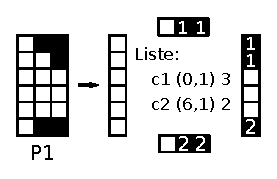
\includegraphics[width=0.6\textwidth]{images/find_result.eps}
	\caption{Beispiel für das (lokale) Ergebnis nach Ausführung der Komponenten-Ermittlung}
	\label{fig:find_result}
\end{figure}

\subsection{Übermittlung der Ergebnisse}

Im letzten Schritt müssen die Ergebnisse der lokalen Ermittlungen so zusammengefügt werden, dass die Komponenten, die durch die Zerteilung aufgeteilt wurden, wieder zusammengefügt werden.

Hierzu überträgt jeder Prozessor sein Ergebnis aus Schritt 2 an seinen direkten Nachbarn (Komponenten-Liste und der angrenzender Rand). Der Nachbar muss dann überprüfen, ob auf den beiden aneinanderliegenden Rändern Komponenten in direkter Nachbarschaft liegen. Falls das der Fall ist, muss eine der beiden Komponenten zur anderen hinzugefügt werden - hier ist nur die Größe relevant - und anschließend muss sie aus der Liste entfernt werden, um nicht doppelt zu erscheinen. Alle Komponenten aus der empfangenen Liste, die nicht mit eigenen Komponenten zusammenhängen werden in die eigene Liste übernommen.

In unserem Beispiel würde Prozessor 2 Komponente 1 und Komponente 2 von Prozessor 1 jeweils zu einer eigenen Komponente hinzufügen. Beide Komponenten würde anschließend gelöscht und nicht weiter zum nächsten Prozessor übertragen. Die eigenen Komponenten von Prozessor 2 wären dann 5 und 7 Pixel groß.

Nachdem die Ergebnisse schließlich beim letzten Prozessor angekommen sind und ausgewertet wurden, steht das Gesamtergebnis fest und wird ausgegeben.

\section{Algorithmen}

\subsection{Matrix-Verteilung}

Um die Matrix vom Root-Prozess an die anderen Prozesse im Cluster zu verteilen, werden im wesentlichen 2 MPI-Aufrufe genutzt zu finden. Die Implementierung ist in der folgenden Datei zu finden:

\begin{lstlisting}[language=C, aboveskip=\baselineskip, basicstyle=\footnotesize\ttfamily, lineskip=0pt]
find_components.c:
	static int mpi_distribute_matrix(struct processor_data *pdata, int *dims, matrix_type *input_matrix)
	static int mpi_working_function(struct processor_data *pdata, int *dims)
\end{lstlisting}

Zuerst werden mittels \verb+MPI_Scatterv+ die Dimensionen der zu übertragenen Matrizen verteilt, die anderen Prozesse im Cluster allozieren daraufhin genügend Speicher für die Matrizen. Danach werden mittels speziell angelegter MPI-Datentypen die einzelnen Matrix-Teile übermittelt (verwendet wird \verb+MPI_Type_vector+, um eine Teilmatrix-Zeile zu adressieren). Durch die verwendeten MPI-Datentypen ist es möglich, dass jeder Matrix-Teil nur eine Sende-Operation benötigt.

Leider ist es bei den verwendeten Datenstrukturen nicht möglich Gruppen-Operationen zu verwenden, um die Matrix-Teile zu senden. Die einzige Operation die in Frage kommen würde, ist \verb+MPI_Scatterv+, aber \verb+scatterv+ verwendet ein unzureichendes Displacement (eine nähere Erläuterung dazu ist an der entsprechenden Stelle im Quell-Code hinterlegt).

\subsection{Komponenten-Ermittlung} \label{algorithm:find_components}

Der wesentliche Teil des Programms ist die Ermittlung der vorhandenen Komponenten in einer (Teil-)Matrix. Die Implementierung des Algorithmus befindet sich im wesentlichen in:

\begin{lstlisting}[language=C, aboveskip=\baselineskip, basicstyle=\footnotesize\ttfamily, lineskip=0pt]
components.c, components.h:
	int find_components(matrix_type *mat, struct component_list **comp_list, vector_type **borders)

helper/{matrixgraph.c, matrixgraph.h}
\end{lstlisting}

\verb+find_components()+ fasst das gegebe Problem der Komponenten-Ermittlung als Graphen-Problem auf. Dazu wird die Matrix in einen Graphen überführt (siehe Abbildung \ref{fig:matrix_graph} auf Seite \pageref{fig:matrix_graph}).

\begin{figure}[tbhp]
	\centering
	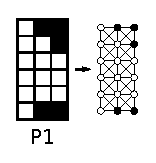
\includegraphics[width=0.4\textwidth]{images/matrix_graph.eps}
	\caption{Beispiel für die Umwandlung einer Matrix in einen Graphen}
	\label{fig:matrix_graph}
\end{figure}

Im überführten Graphen befinden sich dann Knoten mit dem Wert 0 und 1 - für weiß und schwarz. Auf diesen Graphen wird wiefolgt eine Tiefensuche angewendet:

Jeder Knoten erhält eine Farbe (nicht zu verwechseln mit der Farbe der Komponenten; zu Anfang ist jeder Knoten weiß). Danach wird zunächst ein Knoten auf einen Stack gepusht. Mit dieser Push-Operation wird der Knoten außerdem grau gefärbt. Dadurch kann erkannt werden, ob ein Knoten schon auf dem Stack liegt (ohne den Stack zu durchsuchen). Danach läuft der Algorithmus so lange, bis der Stack keine Knoten mehr enthält.

Jede Runde wird ein Knoten vom Stack geholt und expandiert - alle verbundenen Knoten, die noch weiß sind, werden auf den Stack gepusht und es wird untersucht, ob die Knoten den Wert 1 enthalten (also schwarze Pixel in der Matrix sind). Sollte ein Knoten mit Wert 1 vorhanden sein, der noch keiner Komponente zugeordnet ist (die Knoten enthalten neben dem Wert auch die Komponenten-ID), wird eine neue Komponente angelegt und dem Knoten zugeordnet. Außerdem wird eine rekursive Tiefen-Suche gestartet, die das Ziel hat, die neue Komponente zu vervollständigen (\verb+complete_component()+). Als letztes wird der Knoten, der vom Stack geholt wurde, schwarz gefärbt und aus dem Graphen entfernt, somit wird er nie wieder betrachtet. Ein Beispiel für eine solche Expandierung ist in Abbildung \ref{fig:node_expand} auf Seite \pageref{fig:node_expand} zu sehen.

\begin{figure}[tbhp]
	\centering
	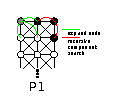
\includegraphics[width=0.5\textwidth]{images/node_expand.eps}
	\caption{Beispiel für das Expandieren eines Knotens}
	\label{fig:node_expand}
\end{figure}

Wenn keine Knoten mehr auf dem Stack sind, ist der Graph komplett durchsucht und alle Komponenten sind gefunden. Da jeder Knoten nur einmal expandiert wird und jeder Knoten eine feste Anzahl von verbundenen Knoten hat (gegeben durch die Entstehung des Graphen), ist die Laufzeit im schlechtesten Fall linear: $O(n*m)$ (in den Messungen, die im Abschnitt \ref{bench:task} auf Seite \pageref{bench:task} vorgestellt werden, kann auch das beobachtet werden).

\subsection{Randabgleich}

Der Abgleich der Rändern zweier aneinanderliegender Matrix-Teile ist in zwei Teile aufgeteilt. Die Implementierung ist aufgeteilt in:

\begin{lstlisting}[language=C, aboveskip=\baselineskip, basicstyle=\footnotesize\ttfamily, lineskip=0pt]
/* Kommunikation */
find_components.c:
	static int mpi_working_function(struct processor_data *pdata, int *dims);

/* Algorithmus zum Abgleich der Raender */
border_compare.c border_compare.h:
	int find_common_components(struct component_list *own_compl, struct component_list *communication_compl, matrix_type *compare_border, matrix_type *send_border, matrix_type *alien_border);
\end{lstlisting}

Zuerst versucht jeder Prozessor von seinem Vorgänger die Daten über dessen lokale Matrix zu erhalten (wie oben schon beschrieben). Im Fall des ersten Prozessors erkennt der Prozessor mittels der angelegten MPI-Topologie und deren Koordinaten, dass er keinen Vorgänger hat und überspringt diese Phase.

\subsubsection{Kommunikation}

Zum Empfangen der Komponenten wird zuerst mittels \verb+MPI_Probe+ und \verb+MPI_get_count+ getestet, wie viele Komponenten übertragen werden sollen (somit reicht eine Sende-Operation, anstelle von zwei, um zuerst die Größe zu übertragen). Beim anschließenden blockierenden \verb+MPI_Recv+ wird ein eigener Typ verwendet, der für die übertragene Struktur angelegt wurde (\verb+MPI_component_type+, angelegt in \verb+register_mpi_component_type()+). Da die Komponenten von Anfang an in einem Vector gespeichert werden (siehe \ref{algorithm:ds} auf Seite \pageref{algorithm:ds}) und deshalb hintereinander im Speicher stehen, reicht eine Sende-Operation und eine einmalige Allozierung auf der Empfänger-Seite aus, um den Austausch der Komponenten abzuschließen.

Der Vorgänger überträgt danach noch den Rand, der an dem des aktuellen Knoten anliegt, damit der aktuelle Knoten zusammenhängende Komponenten erkennen kann (der Rand ist auch eine Matrix, mit nur einer Dimension, und enthält in seinen Feldern die ID der dort erkannten Komponente, siehe Abbildung \ref{fig:find_result} auf Seite \ref{fig:find_result}). Für diese Übertragung wird auch ein eigener MPI-Datentyp angelegt (\verb+border_type+) und es wird eine blockierende Sende-Operation verwendet (\verb$Send + Recv$).

\subsubsection{Abgleich}

Damit die Komponenten erkannt werden, die durch die Teilung der Matrix separiert wurden, wird vom jeweiligen Empfänger die Funktion \verb+find_common_components()+ benutzt. Diese Funktion vergleicht den empfangenen Rand des Vorgängers (ab hier: \textit{links}) mit dem Rand der eigenen Matrix (ab hier: \textit{recht}), der an diesem anliegt. Dabei geht der Algorithmus den linken Rand von oben nach unten durch und vergleicht das aktuelle Feld mit den drei angrenzenden Feldern im rechten Rand.

Bei diesem Vergleich können folgende Fälle auftreten (jeweils, wenn links und rechts eine Komponente gefunden wird):
\begin{itemize}
	\item Die linke Komponente ist bisher noch nicht verbunden worden: die linke Komponente wird zur rechten hinzu addiert und entfernt. Diese Verbindung wird gespeichert.
	\item Die linke Komponente wurde schon einmal verbunden:
		\begin{itemize}
			\item Es liegt bereits eine Verbindung mit der rechten Komponente vor: keine weitere Aktion.
			\item Es liegt noch keine Verbindung mit der rechten Komponente vor: zwei der eigenen Komponenten werden durch die Fremde verbunden. Diese beiden müssen also verbunden werden und eine muss aus der eigenen Liste entfernt werden. Dabei muss beachtet werden, dass die entfernte Komponenten eventuell in dem Rand auftaucht, der an den Nachfolger des Knotens übertragen werden muss.
		\end{itemize}
\end{itemize}

Sobald der Algorithmus fertig ist, sind alle passenden Komponenten verbunden und der Rest der empfangenen Komponenten wird in die eigene Liste übernommen. Die eigene Liste wird danach an den nächsten Knoten versendet. Für den Fall, dass der aktuelle Knoten bereits der letzte ist, steht nun das Ergebnis zur Verfügung.

\subsection{Datenstrukturen} \label{algorithm:ds}

In allen Teilen des Programms wurden einige höhere Datenstrukturen verwendet, die es zum einen erleichtern sollen, den allozierten Speicher des Programms zu verwalten und zum anderen, den Zugriff auf den Speicher zu vereinheitlichen. Da C selbst keine solchen Datenstrukturen in seiner Standard-Bibliothek zur Verfügung stellt, wurden eigene entwickelt. Die Header-Dateien sind in:

\begin{lstlisting}[language=C, aboveskip=\baselineskip, basicstyle=\footnotesize\ttfamily, lineskip=0pt]
helper/vector.h
helper/list.h
helper/matrix.h
helper/stack.h
helper/queue.h
helper/matrixgraph.h /* spezieller Graph fuer dieses Programm */
helper/constvector.h /* spezielle Variante eines vectors, fuer eigene Allokatoren gedacht */
\end{lstlisting}

Verwendet wurden in dem Programm hauptsächlich:

\begin{itemize}
	\item \textsl{\textbf{Vector:}} 'dynamisches' Array. Auf \verb+vector->values+ wird Speicher alloziert (je nach Größe der zu speichernden Elemente), falls durch eine \verb+add+-Operation dieser Speicher überlaufen würde, wird er automatisch erweitert (\verb+realloc+).
	\item \textsl{\textbf{Matrix:}} ein verwaltetes zweidimensionales Array. Auf \verb+matrix->matrix+ wird genügend Speicher für $m \times n$ Elemente der angegebenen Größe alloziert, anschließend kann dieser Speicher nicht geschrumpft/vergrößert werden. Bei Zugriffen werden die Indizes überprüft, um Segmentation-Faults zu vermeiden.
	\item \textsl{\textbf{Stack:}} ein klassischer Stack, basierend auf einem Vector.
	\item \textsl{\textbf{Matrixgraph:}} eine spezielle Graphen-Struktur, die auf eine Matrix aufbaut. Dabei wird die Regelmäßigkeit einer Matrix ausgenutzt, so können Zugriffszeiten linear bleiben.
\end{itemize}

Bei all diesem Datenstrukturen ist zu beachten: Da C keine Form von Polymorphie unterstützt, müssen die Elemente der Strukturen als void-Pointer behandelt werden, da sonst keine allgemeinen Strukturen möglich sind. Das hat aber zur Folge, dass bei \verb+Get/Add/..+ Operationen keine Typ-Prüfung stattfinden kann. Diese Aufgabe muss der Programmierer übernehmen. In den Quelltexten dieses Programms wurde soweit möglich jede verwendete Datenstruktur mit dem gespeicherten Typ kommentiert.

\section{Bemerkungen}

Zu einiges Teilen des Programms gibt es Besonderheiten zu beachten:

\subsection{MPI-Topologie}

Bei der Verteilung der Matrix und der Ergebnisse der Erkennungs-Phase wird eine MPI-Topologie verwendet. Diese ist bei der simplen Aufteilung der Matrix nicht unbedingt nötig. Es war zu Anfang der Implementierung aber die Möglichkeit geplant, die Matrix nicht nur eindimensional zu teile, sondern zweidimensional, dafür wäre die Topologie sehr nützlich. Diese Möglichkeit wurde aber im laufe der Implementierung verworfen, da dadurch die Ermittlung von gemeinsamen Komponenten erheblich komplexer werden würde und damit wesentlich mehr Zeit benötigen würde. In diesem Fall lassen sich Beispiele konstruieren, in denen es nicht mehr ausreicht nur die Ränder der Teil-Matrizen zu vergleichen, man müsste auch die Entstehungs-Geschichte der Komponenten in der Vergangenheit beachten.

\begin{figure}[tbhp]
	\centering
	\includegraphics[width=0.45\textwidth]{images/bordercompare_illegal}
	\caption{Beispiel für eine Matrize die bei zweidimensionaler Einteilung zu falschen Ergebnissen führen kann}
	\label{fig:bcomp_illegal}
\end{figure}

Ein solch konturiertes Beispiel ist in Abbildung \ref{fig:bcomp_illegal} auf Seite \pageref{fig:bcomp_illegal} zu sehen. Verfolgt man hier den Abgleich der Komponenten zwischen den Rändern (von einem Prozessor jeweils nach rechts und nach unten, so dass P9 der letzte Prozessor ist) und würde der Abgleich immer nur die beiden empfangenen Ränder und die eigenen Komponenten betrachten (im Fall von P9 würde man also zwei eigene Komponenten und jeweils eine fremde Komponente auf den Rändern betrachten), dann hätte das zur Folge, dass Prozessor 9 zwei Komponenten als Ergebnis ausgeben würde und nicht eine.

Um diesen komplexen Fall zu erkennen, müsste jede Komponente ihre eigene Entstehungs-Geschichte speichern, also aus welchen Einzel-Komponenten und von welchen Prozessoren sie jeweils zusammengesetzt wurde. Dann könnte Prozessor 9 erkennen, dass die Komponenten von Prozessor 6 und Prozessor 8 auf Prozessor 5 verbunden wurden. Das hat aber zur Folge, dass bei jedem Randabgleich \textbf{alle} Komponenten der verbundenen Prozessoren auf gemeinsame Teile untersucht werden müssten (weil selbst Prozessor 6 kann noch nicht erkennen, dass seine Komponente in Prozessor 5 mit einer anderen verbunden wird). Bei großen Komponenten-Mengen (in unserer Messung, die später noch gezeigt wird, waren es z.B. mehr als $320000$) würde das zu einer hohen Komplexität an Such- und Vergleich-Operationen führen, selbst wenn die Komponenten-Listen sortiert und damit Logarithmisch durchsuchbar sind.

\subsection{Speicheraufwand in der Erkennungsphase}

Die angesprochene lineare Laufzeit der Erkennungsphase wird vor allem dadurch erkauft, das während der Laufzeit alle gesehenen Knoten im Graphen auf einem Stack gespeichert werden. Somit ist kein Backtracking notwendig und der vom Betriebssystem zur Verfügung gestellt Funktions-Stack wird nicht belastet. Das hat aber bei großen Matrizen zur Folge, dass dieser Stack sehr groß werden kann (je nachdem wie die Suche verläuft). Dazu kommt, dass große Matrizen schon so viel Speicher benötigen, damit Komponenten-Bestandteile (ID, Größe, Koordinaten) und Graphen-Farben gespeichert werden können.

Das führt dazu, das dieser Teil des Algorithmus sehr Speicher-Intensiv ist. Was allerdings durch die Cluster-Verarbeitung wieder abgeschwächt werden kann. Der Algorithmus könnte auch mit Backtracking im Graphen realisiert werden, was die Laufzeit-Komplexität aber erheblich anheben würde.

\subsection{Such-Aufwand im Rand-Abgleich}

Beim abgleichen der Ränder zweier Komponenten muss oft auf einzelne Komponenten und gespeicherte Verbindungen zugegriffen werden, um Zusammenhänge zu erkennen (wie oben schon erläutert). Diese Zugriffe geschehen derzeit nicht per Indexierung, weshalb eine Form der Suche angewendet werden muss. Um die Laufzeit davon zu begrenzen werden die Komponenten-Listen und Listen von Verbindungen sortiert, um danach eine binäre Suche anwenden zu können. Trotzdem steigt deswegen die Komplexität dieser Phase an.

Diese Komplexität kann mit komplexeren Datenstrukturen verringert werden. Ein balancierter Baum z.B. würde die Laufzeit vom sortierten Einfügen erheblich verringern (gegenüber dem jetzt verwendeten Vector). Aber dazu müsste auch ein spezieller Allokator implementiert werden, der es ermöglicht gleichzeitig - mit einem malloc - mehrere Baumelemente vor Gebrauch zu reservieren, damit nicht während der Laufzeit für jedes Baumelement einzeln Speicher alloziert werden muss. Bei großen Komponenten-Mengen würde das die Laufzeit explodieren lassen (jedes malloc hat Systemaufrufe zur Folge).

Außerdem könnten die Verbindungen mit geschickter Zeiger-Logik direkt mit den Komponenten verbunden werden, was jeglichen Such-Aufwand eliminieren würde.

Beides wurde wegen dem nötigen Zeitaufwand vorerst zurück gestellt.

\section{Laufzeitanalyse}

Bei den Laufzeitmessungen des Programms wurde eine Matrize mit den Dimensionen $8192 \times 8192$ verwendet. Diese Matrix wurde mit Hilfe des \texttt{pixelpattern}-Generators erstellt und enthielt $321413$ Komponenten, die im Schnitt $87.5$ Pixel groß waren (der Generator wird näher bei \ref{pixelpattern} auf Seite \pageref{pixelpattern} beschrieben).

Bei den Messungen wurde das Programm jeweils mit $1$, $2$, $4$ und $8$ Prozessoren ausgeführt. Für jede Anzahl der Prozessoren wurden $10$ Programmdurchläufe gemacht, um Schwankungen auszuschließen (wie man in den Messergebnissen sehen kann, waren die Schwankungen nicht sehr groß).

\subsection{Gesamtlaufzeit} \label{bench:whole}

In Abbildung \ref{fig:bench_whole} auf Seite \pageref{fig:bench_whole} sind die Gesamtlaufzeiten für die gemessenen Prozessor-Kombinationen zu sehen.

\begin{figure}[tbhp]
	\centering
	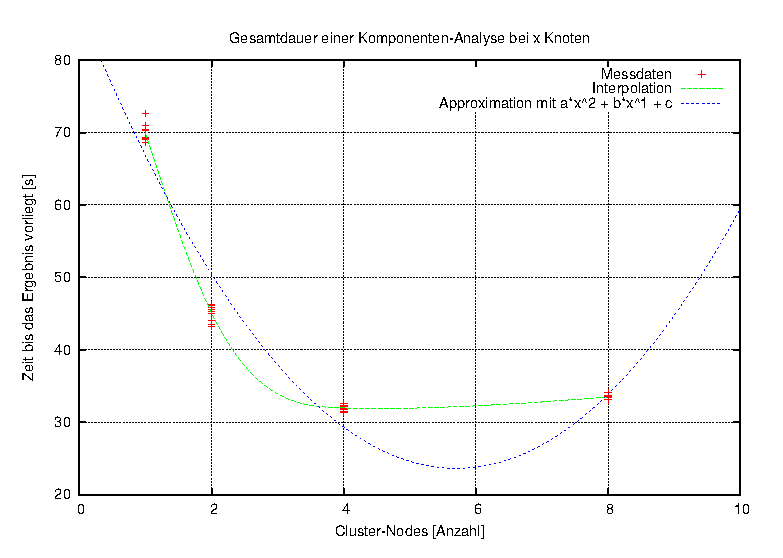
\includegraphics[width=0.9\textwidth]{images/whole_plod.eps}
	\caption{Messung der Gesamtlaufzeit}
	\label{fig:bench_whole}
\end{figure}

Wie man sieht, nimmt die Laufzeit bis zu einer Cluster-Größe von 4 Prozessoren stetig ab, um dann bei einer Größe von 8 wieder anzusteigen. Die angegeben Interpolation der Messwerte gibt dabei die Laufzeit besser wieder, als die Approximation (bei einer weiteren Testmessung mit 6 Prozessoren wurde keine wesentliche Verbesserung zu 4 Prozessoren festgestellt).

\subsection{Laufzeiten der Einzel-Aufgaben} \label{bench:task}

Warum die Gesamtlaufzeit bei 8 Prozessoren wieder steigt ist in Abbildung \ref{fig:bench_tasks} auf Seite \pageref{fig:bench_tasks} gut zu sehen. Hier werden jeweils die Laufzeiten der einzelnen Aufgaben dargestellt.

\begin{figure}[tbhp]
	\centering
	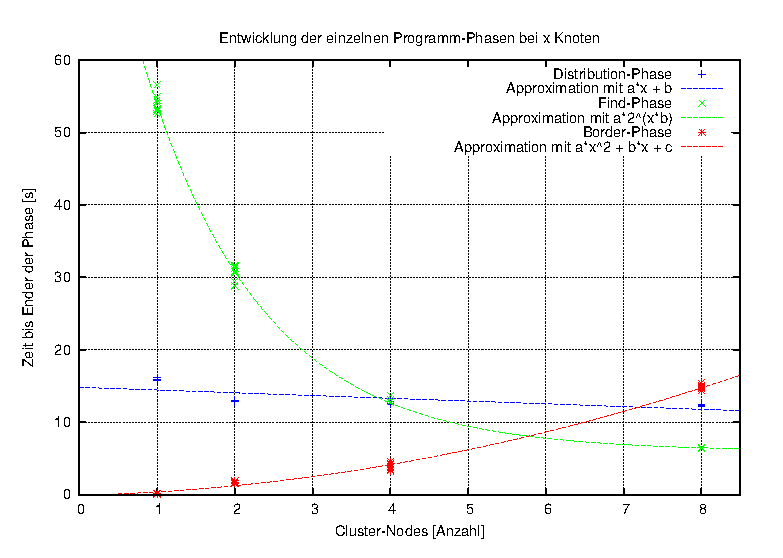
\includegraphics[width=0.9\textwidth]{images/phases.eps}
	\caption{Messung der Laufzeit der einzelnen Aufgaben}
	\label{fig:bench_tasks}
\end{figure}

Zu sehen ist, dass die Verteilung der Matrix im wesentliche gleich bleibt, die Laufzeit dieser Phase ist wesentlich durch das Einlesen der Matrix vom Dateisystem und der Geschwindigkeit des Netzwerks zur Übertragung beschränkt. Insgesamt müssen $192MByte$ von der Festplatte gelesen werde und ca. $48MByte$ übertragen werden (die genaue Größe bei der Übertragung hängt natürlich von der Größe des Clusters ab, da dann die Matrizen anders dimensioniert werden).

Was auch gut zu sehen ist, ist das lineare Laufzeitverhalten der lokalen Erkennungsphase, halbiert sich die Größe der lokalen Matrix, halbiert sich auch die Laufzeit der Erkennungsphase.

Schließlich übersteigen die Kosten der letzten Programm-Phase aber die, der Einsparung in der Erkennungsphase. Der Grund dafür ist offensichtlich. Je größer der Cluster wird, desto öfter müssen Ränder abgeglichen werden und desto länger muss der letzte Prozess warten, bis er das Ergebnis vorliegen hat. Außerdem steigt die Anzahl der übermittelten Komponenten bei jedem Prozessor an (begründet durch die hohe Anzahl in der Test-Matrix), dadurch steigt der Aufwand im Abgleich der Komponenten.

\section{Pixelpattern-Generator}

\label{pixelpattern}

Neben dem eigentlichen Hauptprogramm wurde außerdem ein Generator entwickelt, der genutzt werden kann, um zufällige Eingabe-Matrizen für das Hauptprogramm zu erzeugen. Dieser soll hier nicht im vollen Umfang beschrieben werden, aber die nötigen Einstellungen, um die generierten Muster anzupassen.

Die Implementierung des Generators befindet sich in:

\begin{lstlisting}[language=C, aboveskip=\baselineskip, basicstyle=\footnotesize\ttfamily, lineskip=0pt]
pixelpattern.c
\end{lstlisting}

Der Generator wird mit der Größe der zu generierenden Matrix aufgerufen. Die Parameter der Muster müssen derzeit noch im Quelltext selbst angepasst werden. Dabei kann folgendes beeinflusst werden (\verb+pixelpattern.c:main():79+):

\begin{itemize}
	\item \textsl{\textbf{filling:}} zu welchem Grad die Matrix mit schwarzen Pixel gefüllt werden soll (es kann bei hohen Graden vorkommen, dass der Generator früher abbricht).
	\item \textsl{\textbf{failcount:}} wenn der Generator eine neue Komponente anlegen will, sucht er eine zufällige Position in der zu dem Zeitpunkt vorhandenen Matrix, falls diese Position zu nah an einer bereits vorhandenen Komponente liegen sollte, wird erneut eine Postion gewählt. Dieser Vorgang bricht ab, sobald der \verb+failcount+ erreicht ist.
	\item \textsl{\textbf{bulginess:}} gibt die Form der Komponenten an, je größer die Zahl ist, desto wahrscheinlicher ist es, dass die Komponente ein "`Pixelhaufen"' wird. (Hängt auch von der \verb+dist+ ab)
	\item \textsl{\textbf{dist:}} gibt an, wie viele Pixel zwei Komponenten mindestens entfernt sein müssen.
	\item \textsl{\textbf{size:}} beeinflusst, wie groß eine Komponente durchschnittlich werden soll. Je kleiner diese Zahl wird, desto größer werden die Komponenten. Bsp.: wenn \verb+size = 1+ ist, dann reduziert sich die Wahrscheinlichkeit, das eine Komponente um einen Pixel erweitert wird je bereits vorhandenem Pixel um $1\%$.
\end{itemize}

Wenn Pixelpattern zum Beispiel mit folgenden Einstellungen gebaut wird:

\begin{lstlisting}[language=C, aboveskip=\baselineskip, basicstyle=\footnotesize\ttfamily, lineskip=0pt]
[...]
int
main(int argc, char ** argv)
{
        long int width, height;
        double filling = 0.25;
        unsigned int failcount = 500,
                     bulginess = 3,
                     dist = 1;
        double       size = 5;
[...]
\end{lstlisting}

dann würden Matrizen generiert, die annähernd zu einem Viertel mit schwarzen Pixeln gefüllt sind, dabei würde der Generator erst nach 500 Fehlversuchen, eine neue Komponente zu platzieren, abbrechen. Die generierten Komponenten würden wahrscheinlich keine große Anhäufungen von direkt nebeneinanderliegenden Pixeln enthalten. Sie würden mindestens 1 Pixel voneinander entfernt sein und durchschnittlich 10 Pixel groß (nach 10 Pixeln sinkt die Wahrscheinlichkeit eines neuen Pixels auf $50\%$).

\end{document}
